\section[A global function on Y]{A global function on \(Y\)} \label{sec:global-func}
We remind the reader of our convention that \(\pi_{x,y}=\pi_{y,x}^{-1}\).
Let us rephrase \pref{cor:good-cocycle}.
\begin{lemma} \label{lem:good-exact-cover}
    There exists a cocycle \(\psi \in Z^1(X,Sym(\ell))\) such that \(\Prob[s_1,s_2, t=s_1 \dunion s_2]{\psi(s_1, s_2)=\pi_{t,s_2}^{-1} \circ \pi_{t_1,s_1} } = 1-\exp(-\Omega(d_1/k)),\) where \(\pi_{t,s_i}\) are the permutations over the list of functions of \(s_i\) and \(t\) respectively as in \pref{lem:from-1-percent-to-list-agreement}.
\end{lemma}
Let us denote the \(\ell\)-cover that this cocycle induces by \(\rho:Y\to X\) such that we have an isomorphism $\iota:\FX{d_1}Y\to\widetilde{\FX{d_1}X}$. 
Recall that we defined, in Section \ref{sec:globalfunc},
functions \(h_{\tilde{s}}:\tilde{s} \to \Sigma\) by
\begin{equation}
    h_{\tilde{s}}((v,i))=L_s^j(\rho(v,i))=L_s^j(v)
\end{equation}
where \(\iota(\tilde{s})=(s,j)\). Using these functions we defined \(G:Y(0) \to \Sigma\) via \(G(v,i)=plurality \sett{ h_{\tilde{s}}((v,i))}{(v,i) \in \tilde{s}}\), i.e. the most popular assignment of \((v,i)\) from all the \(h_{\tilde{s}}\) where \(\tilde{s} \ni (v,i)\).

The final component we need for proving our main theorem is that most \(h_{\tilde{s}}\) agree with \(G\) on most vertices.
\restateclaim{claim:agreement-with-majority}

For the proof of the lemma, we need the following agreement theorem taken from \cite{DiksteinH2023}.
\begin{theorem}[{\cite[Claim 8.5]{DiksteinH2023}}]\label{thm:agreement-high-acceptance}
    There exists a universal constant \(c>0\) such that the following holds. Let \(Y\) be a \(\frac{1}{d_1^3}\)-one sided high dimensional expander. Let \(DU_n\) be the \((d_1,\frac{3}{2}d_1)\)-non-lazy-up-down walk in \(Y\) as in \pref{def:non-lazy-up-down}. Let \(\mathcal{H}=\set{h_{\tilde{s}}}_{\tilde{s} \in Y(d_1)}\) be an ensemble of functions such that
    \[\Prob[\tilde{s}_1,\tilde{s}_2 \sim DU_n]{h_{\tilde{s}_1}|_{\tilde{s}_1 \cap \tilde{s}_2} \overset{1-\eta}{\approx} h_{\tilde{s}_2}|_{\tilde{s}_1 \cap \tilde{s}_2} } \geq 1-\gamma,\]
    then 
    \[\Prob[\tilde{s} \in Y(d_1)]{G|_{\tilde{s}} \overset{1-8(\eta + \gamma)}{\approx} h_{\tilde{s}}} \geq 1-\frac{1}{d_1^c}-\gamma^c.\]
\end{theorem}

\begin{proof}[Proof of \pref{claim:agreement-with-majority}]
\begin{figure}
    \centering
    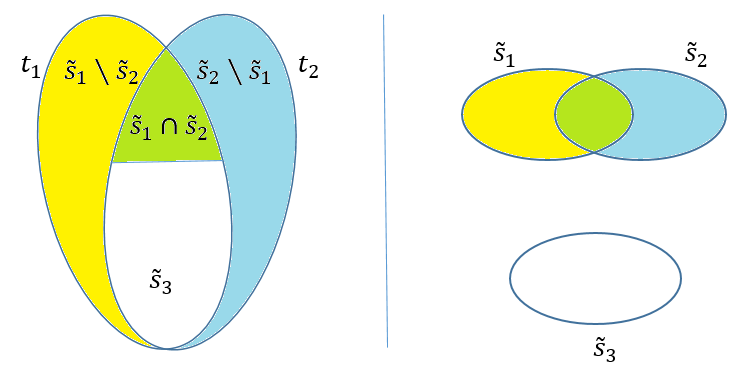
\includegraphics[scale=0.6]{images/set-for-agreement.png}
    \caption{The sets sampled by \(P\). Note that \(\tilde{s_1}\) is the yellow and green parts, \(\tilde{s_1}\) is the blue and green parts, and the \(\tilde{t_i}\)'s are the \(s_i\)'s together with \(\tilde{s_3}\) (the white part which is disjoint from \(\tilde{s_1}\) and \(\tilde{s_2}\)).}
    \label{fig:dist-P}
\end{figure}
    We want to use \pref{thm:agreement-high-acceptance}, and thus we need to show that
    \[\Prob[\tilde{s}_1,\tilde{s}_2 \sim DU_n]{h_{\tilde{s}_1}|_{\tilde{s}_1 \cap \tilde{s}_2} \overset{1-O(\eta)}{\approx} h_{\tilde{s}_2}|_{\tilde{s}_1 \cap \tilde{s}_2} } \geq 1-\exp(-\Omega(d_1/k)),\]

    Let us define the distribution \((\tilde{s}_1,\tilde{s}_2,\tilde{s}_3) \sim P\) where:
    \begin{enumerate}
        \item \(\tilde{s_1}\) and \(\tilde{s_2}\) are sampled via the non-lazy-up-down-walk. That is, \(\tilde{s_1} \cup \tilde{s}_2 \in X(\frac{3}{2}d_1)\).
        \item \(\tilde{s}_3 \dunion (\tilde{s_1} \cup \tilde{s}_2) \in X\), i.e. \(\tilde{s}_3\) is sampled via a swap walk step from \((\tilde{s_1} \cup \tilde{s}_2)\).
    \end{enumerate}
    Let us denote by \(\tilde{t_i} = \tilde{s_i} \dunion \tilde{s_3}\) for \(i=1,2\), and let us denote \(\tilde{r} = \tilde{s}_1 \cap \tilde{s}_2\). See \pref{fig:dist-P} for an illustration of the sets sampled. We also use the convention that \(\rho(\tilde{s}_i) = s_i, \rho(\tilde{t_i})=t_i, \rho(\tilde{r})=r\) (hopefully, it will also be clear from context which faces belong to \(Y\) and which belong to \(X\)).
    
    Let \(j_i\) be the index that has that \(L_{s_i}^{j_i}\circ \rho = h_{\tilde{s_i}}\) for \(i=1,2,3\).  and let \(j_i' = \pi_{t_i,s_i}(j_i)\). We define the following two ``bad'' events
    \begin{enumerate}
        \item \(E = \set{L_{s_i}^{j_i} \overset{1-\eta}{\napprox} L_{t_i}^{j_i'}|_{s_i} \text{ or } L_{s_3}^{j_3} \overset{1-\eta}{\napprox} L_{t_i}^{j_i'}|_{s_3} \text{ for } i=1 \text{ or } i=2}\).
        \item \(F = \set{L_{t_1}^{j_1'}|_{s_3} \overset{1-2\eta}{\approx} L_{t_2}^{j_2'}|_{s_3} \ve L_{t_1}^{j_1'}|_{r} \overset{1-9\eta}{\napprox} L_{t_2}^{j_2'}|_{r}}\).
    \end{enumerate}
    Let us spell out these events. The event \(E\) considers the lists of \(s_1,s_2,s_3\) and \(t_1,t_2\). The first statement in the event, i.e. that \(L_{s_i}^{j_i} \overset{1-\eta}{\napprox} L_{t_i}^{j_i'}|_{s_i}\), roughly states that at least one of the \(i=1,2\), the lists of \(s_i\) and \(t_i\) are not compatible (at a specific index \(j_i\)). The second statement, namely that \(L_{s_3}^{j_3} \overset{1-\eta}{\napprox} L_{t_i}^{j_i'}|_{s_3}\) is the event that for at least one of the \(i=1,2\), the entry of \(j_3\) in \(s_3\)'s list, is not compatible with \(j_i'=\pi_{t,s_i}(j_i)\). We will see that with very high probability \(j_3 = \pi_{s_3,t}(j_i')\) so this part also essentially says that the one of the lists of \(t_i\) and \(s_3\) are not compatible with one another.
    
    The event \(F\) says that ``even though'' \(L_{t_1}^{j_1'}\) and \( L_{t_2}^{j_2'}\) agree on most vertices of \(s_3\), they do not agree on most vertices of \(r\), the other part of their intersection.

    We claim that both events happen with only small probability (and prove this later on in this section):
    \begin{claim} \label{claim:E-is-small}~ 
        \(\prob{E} \leq \exp(-\Omega(d_1/k))\).
    \end{claim}
    \begin{claim} \label{claim:F-is-small}~ 
        \(\prob{F} \leq \exp(-\Omega(d_1))\).
    \end{claim}
    Let us explain why
    \begin{equation}
        \prob{h_{\tilde{s_1}} \overset{1-13\eta}{\napprox} h_{\tilde{s_2}}} \leq \prob{E} + \prob{F} = \exp(-\Omega(d_1/k)),
    \end{equation}
    or in other words, why when \(\neg E \ve \neg F\) occur, then \(h_{\tilde{s_1}} \overset{1-13\eta}{\approx} h_{\tilde{s_2}}\).
    
    Indeed, if \(E\) doesn't occur then for \(i=1,2\), \(L_{s_i}^{j_i} \overset{1-\eta}{\approx} L_{t_i}^{j_i'}|_{s_i}\),  and thus it holds that \(L_{s_i}^{j_i}|_r \overset{1-2\eta}{\approx} L_{t_i}^{j_i'}|_r\) (since \(r\) is at \(\frac{1}{2}\) the size of \(\tilde{s_i}\) for both \(i=1,2\)). For similar reasons, \(L_{t_1}^{j_1'}|_{s_3} \overset{1-\eta}{\approx} L_{s_3}^{j_3} \overset{1-\eta}{\approx} L_{t_2}^{j_2'}|_{s_3}\) and hence \(L_{t_1}^{j_1'}|_{s_3} \overset{1-2\eta}{\approx} L_{t_2}^{j_2'}|_{s_3}\). By \(\neg F\) this implies that \(L_{t_1}^{j_1'} |_r \overset{1-9\eta}{\approx} L_{t_2}^{j_2'}|_r\). In total, it holds that
    \[h_{\tilde{s_1}}|_{\tilde{r}} = (L_{s_1}^{j_1} \circ \rho)|_{\tilde{r}} \overset{1-2\eta}{\approx} (L_{t_1}^{j_1'} \circ \rho)|_{\tilde{r}} \overset{1-9\eta}{\approx} (L_{t_2}^{j_2'} \circ \rho)|_{\tilde{r}} \overset{1-2\eta}{\approx} L_{s_1}^{j_2'} \circ \rho|_{\tilde{r}} = h_{\tilde{s_2}}|_{\tilde{r}},\]
    so \(h_{\tilde{s_1}}|_{\tilde{r}} \overset{1-13\eta}{\approx} h_{\tilde{s_2}}|_{\tilde{r}}\). The claim follows from \pref{thm:agreement-high-acceptance}.
\end{proof}

\begin{proof}[Proof of \pref{claim:E-is-small}]
Let us begin with bounding the probability that \(L_{s_i}^{j_i} \overset{1-\eta}{\napprox} L_{t_i}^{j_i'}|_{s_i}\) for some \(i=1,2\). We note that \(s_i,t_i\) are chosen according to the usual joint distribution of \((s\subset t)\) in \(X\). Thus the probability that \(\prob{L_{s_i}^{j_i} \overset{1-\eta}{\napprox} L_{t_i}^{j_i'}}\) for both \(i=1,2\) is at most
\[1-\Prob[t\in X(\frac{3}{2}d_1),s\subset t, s\in X(d_1)]{\forall j=1,2,...,\ell, \; L_s^j \overset{1-\eta}{\approx} L_t^{\pi_{t,s}(j)}|_s} = \exp(-\Omega(d_1/k))\]
by \pref{lem:from-1-percent-to-list-agreement}. When this occurs then \(L_{s_i}^{x} \overset{1-\eta}{\approx} L_{t_i}^{\pi_{t_i,s_i}(x)}|_{s_i}\) for all indexes \(x\), and in particular for \(j_i\).

We move towards bounding the probability that \(L_{s_3}^{j_3} \overset{1-\eta}{\napprox} L_{t_i}^{j_i'}|_{s_3}\) for some \(i=1,2\). The pair \(s_3,t_i\) is also distributed according to the joint distribution of \((s\subset t)\) in \(X\). Hence it holds that \(\prob{L_{s_3}^{j_3} \overset{1-\eta}{\napprox} L_{t_i}^{\pi_{t_i,s_3}(j_3)}} = \exp(-\Omega(d_1/k))\).

Moreover, by \pref{lem:good-exact-cover}, with probability \(1- \exp(-\Omega(d_1/k))\) it holds that \(\psi(s_i, s_3)=\pi_{t_i,\tilde{s_3}}^{-1} \circ \pi_{t_i,\tilde{s_i}}\) (where \(\psi\) is the cocycle that defined the cover \(\rho\)). Recall that \(\iota(\tilde{s_i})=(s_i,j_i)\) where \(\iota:\FX{d_1}Y \to \widetilde{\FX{d_1}X}\) and \(\tilde{s_i},\tilde{s_3} \in \FX{d_1}Y(0)\) are neighbors in \(\FX{d_1}Y\) which implies that for \(i=1,2\), \((s_i,j_i) \sim (s_3,\psi(s_i,s_3) . j_i)\) are neighbors in \(\widetilde{\FX{d_1}X}\). Thus with probability \(1- \exp(-\Omega(d_1/k))\), 
\[j_3 = \pi_{t_i,s_3}^{-1} \circ \pi_{t_i,s_i}(j_i)\]
for \(i=1,2\). When this occurs, then
\[\pi_{t_i,s_3}(j_3) = \pi_{t_i,s_i}(j_i)=j_i',\]
and as above \(\prob{L_{s_3}^{j_3} \overset{1-\eta}{\napprox} L_{t_i}^{j_i'}|_{s_3}} \leq \exp(-\Omega(d_1/k))\).

\end{proof}

The proof of \pref{claim:F-is-small} is just by basic probabalistic arguments, and doesn't rely on any of the machinery we developed.
\begin{proof}[Proof of \pref{claim:F-is-small}]
    Fix any \(t_1,t_2\), and denote \(t' = t_1 \cap t_2\). Fix any \(f=L_{t_1}^{j_1'}|_{t'}, g=L_{t_2}^{j_2'}|_{t'}:t' \to \Sigma\). The choice of \(r, s_3 \subseteq t'\) is uniform among all pairs such that \(r \dunion s_3 = t'\). We will show that
    \[\Prob[\tilde{s_3},r]{f|_{s_3} \overset{1-2\eta}{\approx} g|_{s_3} \ve f|_{r} \overset{1-9\eta}{\napprox} g|_{r}} \leq \exp(-\Omega(\eta^2 |s|))\]
    which proves the claim since \(|s| =\Omega(d_1)\) and \(\eta\) is a constant.
    
    Indeed, if \(f|_{r} \overset{1-9\eta}{\napprox} g|_{r}\), then \(f \overset{1-3\eta}{\napprox} g\) (since \(r\) is a third of the size of \(t'\)). In this case, the probability of choosing \(s_3 \subseteq t'\) of size greater or equal to half of \(t'\) such that \(L_{t_1}^{j_1'}|_{s_3} \overset{1-2\eta}{\approx} L_{t_2}^{j_2'}|_{s_3}\) is at most \(\exp(-\Omega(\eta^2 d_1))\) by a standard Chernoff bound.
\end{proof}
